\section{Servidor gRPC}

El servidor gRPC es el componente de cada nodo que recibe los mensajes de los
demás nodos. Implementa la única función remota que declara el contrato,
\texttt{EnviarMensaje(Mensaje) returns (Acuse)}, y cumple el mismo papel que
\texttt{tcp\_server.py} en la implementación TCP: recibe un mensaje, actualiza
el reloj de Lamport, registra los eventos y responde con una confirmación. El
código está en \texttt{src/grpc/grpc\_server.py}, y cada nodo
(\texttt{nodo-A}, \texttt{nodo-B} y \texttt{nodo-C}) se inicia con su propia
dirección y puerto.

\subsection{Estructura del servidor}

La clase \texttt{ComunicacionNodosServicer} hereda de
\texttt{servicio\_pb2\_grpc.ComunicacionNodosServicer}, la clase base generada
a partir del \texttt{service} del archivo \texttt{.proto}. Su constructor
recibe tres datos y los guarda: el nombre del nodo (\texttt{node\_name}), su
reloj de Lamport (\texttt{clock}) y su registrador de eventos (\texttt{logger}).
Al recibirlos desde fuera, la clase no depende de cómo se crean, y la misma
lógica se puede reutilizar para los tres nodos.

La función \texttt{create\_server} arma el servidor: crea un
\texttt{grpc.server} con un \texttt{ThreadPoolExecutor} de 10 hilos
(\texttt{max\_workers=10}), registra el \emph{servicer} con
\texttt{add\_ComunicacionNodosServicer\_to\_server} y abre el puerto con
\texttt{add\_insecure\_port}. El \texttt{ThreadPoolExecutor} es lo que permite
atender varias llamadas a la vez: cada llamada que llega se ejecuta en un hilo
del grupo, de modo que, mientras una se procesa, otra puede empezar sin esperar
a que la primera termine, hasta un máximo de 10 simultáneas.

Esto marca una diferencia con la versión TCP. \texttt{TCPNodeServer} hereda de
\texttt{ThreadingTCPServer}, que crea un hilo nuevo por cada conexión sin
ningún límite, mientras que el servidor gRPC usa un grupo fijo de 10 hilos. El
grupo acota el número de hilos y, por tanto, el consumo de recursos, pero si
llegan más de 10 llamadas a la vez, las demás esperan a que se libere un
hilo.

\begin{figure}[htbp]
  \centering
  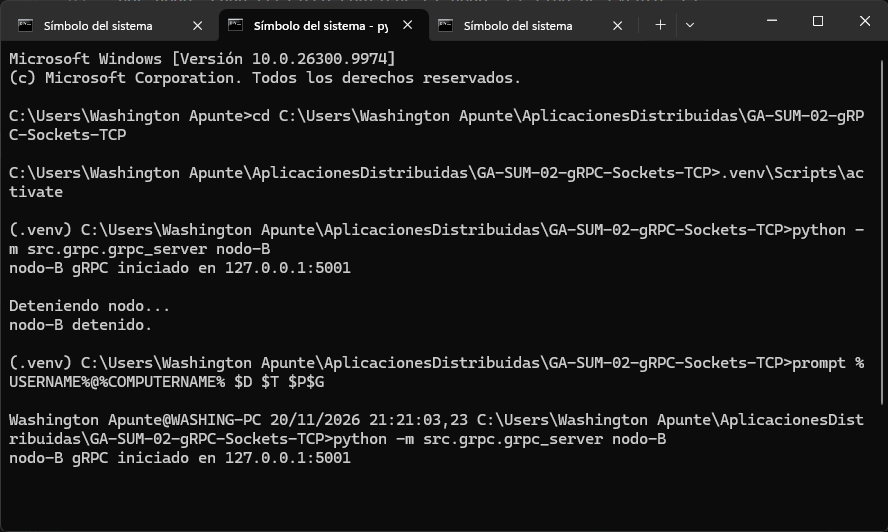
\includegraphics[width=\linewidth]{informe/capturas/captura_servidor.png}
  \caption{Inicio de un nodo del servidor gRPC.}
  \label{fig:servidor}
\end{figure}

\subsection{Qué hace \texttt{EnviarMensaje}}

Cada llamada ejecuta los siguientes pasos, en este orden:

\begin{enumerate}
  \item Validar la solicitud: se comprueba que el emisor no esté vacío y que
        el \texttt{timestamp} no sea negativo. Si algo falla, se rechaza la
        llamada y no se ejecuta ningún paso más.
  \item Llamar a \texttt{clock.after\_receive(request.timestamp)} para
        actualizar el reloj con el valor recibido, y registrar el evento
        \texttt{receive} con el valor que devuelve.
  \item Llamar a \texttt{clock.before\_send()} para incrementar el reloj antes
        de responder, y registrar el evento \texttt{send} con ese valor.
  \item Devolver un \texttt{Acuse} con el nombre del nodo como
        \texttt{sender}, el valor del paso 2 en \texttt{received\_timestamp},
        el valor del paso 3 en \texttt{timestamp} y el mensaje
        \texttt{"ACK: "} seguido del texto recibido.
\end{enumerate}

\begin{figure}[htbp]
  \centering
  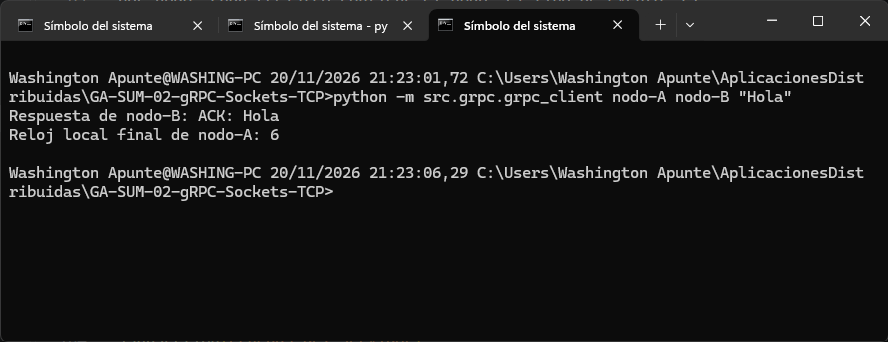
\includegraphics[width=\linewidth]{informe/capturas/captura_cliente.png}
  \caption{El cliente envía un mensaje y recibe el acuse del servidor.}
  \label{fig:cliente}
\end{figure}

\subsection{Validación y errores}

El servidor rechaza dos casos: un emisor vacío, con el mensaje
\texttt{"Emisor invalido"}, y un \texttt{timestamp} negativo, con el mensaje
\texttt{"Timestamp invalido"}. En ambos usa
\texttt{context.abort(grpc.StatusCode.INVALID\_ARGUMENT, \dots)}, que
interrumpe la función, de modo que no hace falta un \texttt{return}. En
\texttt{proto3} un campo \texttt{string} que no se envía llega como cadena
vacía, por lo que la misma comprobación cubre el emisor vacío y el emisor
ausente.

Los tipos de los campos ya los garantiza el contrato, por eso no se repiten
las comprobaciones de tipo que sí hace \texttt{tcp\_server.py}
(\texttt{isinstance} para \texttt{sender} y \texttt{message}, y
\texttt{type(timestamp) is not int} para el \texttt{timestamp}; esta última
forma también rechaza los valores booleanos). Del lado del cliente, la llamada rechazada se manifiesta
como una excepción \texttt{grpc.RpcError} con el código
\texttt{INVALID\_ARGUMENT} y el texto del error. Es el equivalente a la
respuesta \texttt{\{"error": \dots\}} de la versión TCP. Como la validación
ocurre antes de tocar el reloj, una solicitud rechazada no modifica el reloj
ni deja eventos registrados.

\begin{figure}[htbp]
  \centering
  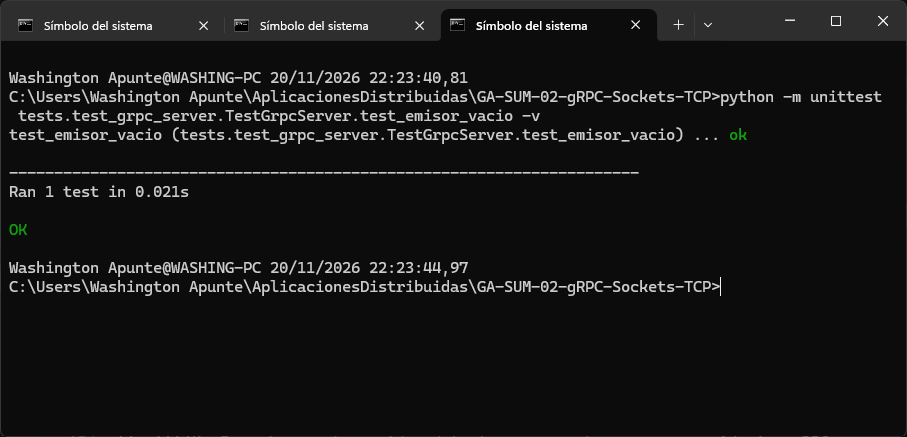
\includegraphics[width=\linewidth]{informe/capturas/captura_emisor_vacio.png}
  \caption{Prueba \texttt{test\_emisor\_vacio}: el servidor rechaza un emisor vacío.}
  \label{fig:vacio}
\end{figure}

\begin{figure}[htbp]
  \centering
  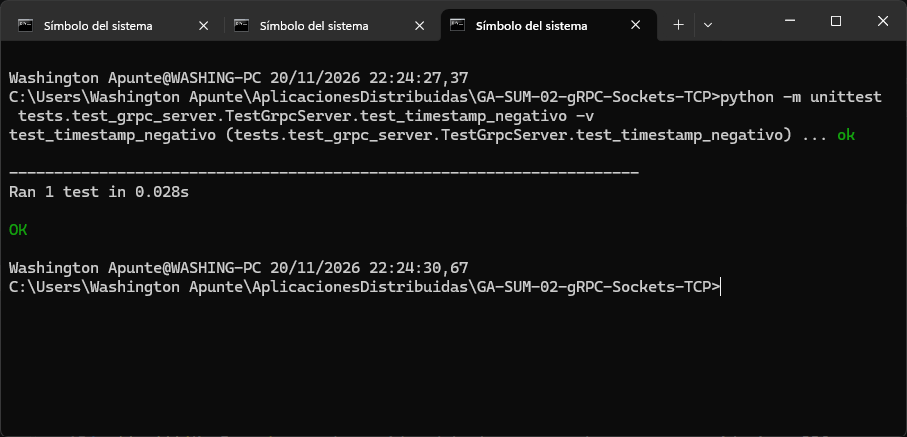
\includegraphics[width=\linewidth]{informe/capturas/captura_timestamp_negativo.png}
  \caption{Prueba \texttt{test\_timestamp\_negativo}: el servidor rechaza un \texttt{timestamp} negativo.}
  \label{fig:negativo}
\end{figure}

\subsection{Reloj de Lamport y registro de eventos}

El reloj de Lamport~\cite{lamport1978} se actualiza en dos puntos de \texttt{EnviarMensaje}:
\texttt{after\_receive} al recibir, que tiene en cuenta el \texttt{timestamp}
del emisor, y \texttt{before\_send} antes de responder. Por cada llamada
aceptada, el servidor registra dos eventos con \texttt{logger.log\_event}: uno
de tipo \texttt{receive} y otro de tipo \texttt{send}, ambos con el nombre del
nodo y el valor del reloj en ese momento.

Los eventos se escriben en \texttt{data/grpc\_events\_\textless{}nodo\textgreater{}.csv}, un archivo
por nodo. Cada registro contiene el nodo, el tipo de evento, el
\texttt{timestamp} de Lamport y la fecha y hora reales, igual que en la
implementación TCP, lo que permite comparar los dos mecanismos con el mismo
formato de datos.

Como el servidor atiende varias llamadas a la vez, el acceso concurrente al
reloj y al archivo es importante. Cada operación del reloj
(\texttt{time}, \texttt{before\_send} y \texttt{after\_receive}) está protegida
con un \texttt{Lock}, por lo que dos hilos no pueden obtener el mismo valor, y
el registrador de eventos usa otro \texttt{Lock} al escribir en el archivo. Sin
embargo, \texttt{EnviarMensaje} completo no es atómico: dos llamadas
simultáneas pueden intercalar sus pasos, de modo que los eventos de ambas
pueden aparecer mezclados en el CSV, aunque cada valor del reloj sigue siendo
único.

\begin{figure}[htbp]
  \centering
  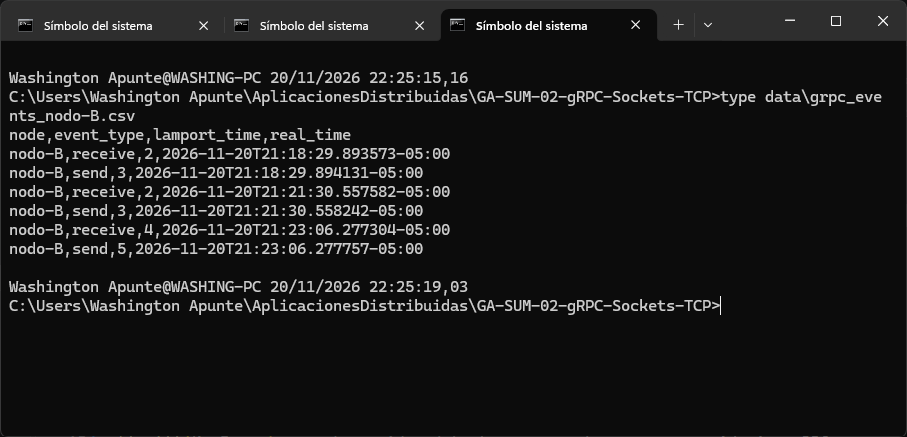
\includegraphics[width=\linewidth]{informe/capturas/captura_csv_eventos.png}
  \caption{Eventos \texttt{receive} y \texttt{send} registrados por \texttt{nodo-B}.}
  \label{fig:csv}
\end{figure}

\subsection{Pruebas del servidor}

Las pruebas del servidor están en \texttt{tests/test\_grpc\_server.py} y se
ejecutan con:

\begin{verbatim}
python -m unittest tests.test_grpc_server -v
\end{verbatim}

El archivo contiene 6 pruebas:

\begin{itemize}
  \item \texttt{test\_timestamp\_negativo}: comprueba que el servidor rechaza
        un \texttt{timestamp} negativo con \texttt{INVALID\_ARGUMENT} y que no
        se registra ningún evento.
  \item \texttt{test\_llamada\_valida}: envía un mensaje con \texttt{timestamp=5}
        y comprueba que la respuesta trae el nombre del nodo, el valor de
        reloj 6 al recibir, el valor 7 al responder y el texto
        \texttt{"ACK: hola"}.
  \item \texttt{test\_emisor\_vacio}: envía un mensaje con el emisor vacío y
        comprueba que se rechaza con \texttt{INVALID\_ARGUMENT} y que no se
        registra ningún evento.
  \item \texttt{test\_reloj\_crece\_entre\_llamadas}: hace dos llamadas seguidas y
        comprueba que el valor \texttt{received\_timestamp} de la segunda
        respuesta es mayor que el valor \texttt{timestamp} de la primera.
  \item \texttt{test\_registra\_receive\_y\_send}: hace una llamada con
        \texttt{timestamp=5} y comprueba que el registrador guarda exactamente
        2 eventos: \texttt{receive} con valor 6 y \texttt{send} con valor 7.
  \item \texttt{test\_concurrencia}: prueba de concurrencia. Se lanzaron 30 llamadas desde 10 hilos y no se repitió ningún
        \texttt{timestamp}. Esto demuestra que
        los valores del reloj no se repiten, no que las llamadas sean
        atómicas.
\end{itemize}

\begin{figure}[htbp]
  \centering
  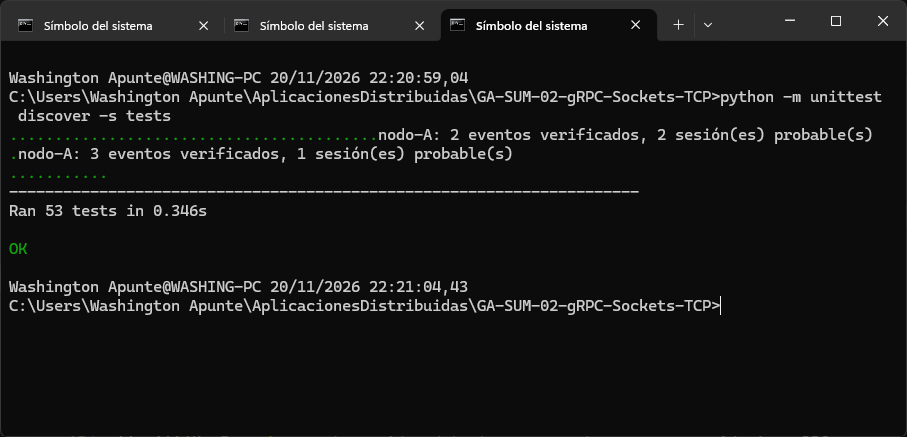
\includegraphics[width=\linewidth]{informe/capturas/captura_53_pruebas.png}
  \caption{Ejecución de las pruebas con \texttt{unittest}: todas pasan.}
  \label{fig:pruebas}
\end{figure}